\documentclass[10pt,twocolumn,twoside]{fernandes_paper} 
%Default opts:9pt,twocolumn,twoside
\graphicspath{{images_paper/}}

\newcommand{\mf}[1]{\colorbox{blue!10}{\color{color3}#1}}

\title{Utilizing Design Principles from Glass Sponges for Structurally Robust Lattices}

\author[1]{Matheus C. Fernandes}
\author[2]{James C. Weaver}
\author[1,2,3]{Joanna Aizenberg}
\author[1,2,3,*]{Katia Bertoldi}

\affil[1]{John A. Paulson School of Engineering and Applied Sciences -- Harvard University, Cambridge, MA 02138}
\affil[2]{Wyss Institute -- Harvard University, Cambridge, MA 02138}
\affil[3]{Kavli Institute -- Harvard University, Cambridge, MA 02138}
\affil[*]{Corresponding author: \href{mailto:bertoldi@seas.harvard.edu}{bertoldi@seas.harvard.edu}}

\keywords{Architected materials, truss structure, buckling resistance, glass sponges, bio-inspired engineering.}

\usepackage{comment}

\begin{document}
\maketitle
% \doublespace
%\linenumbers

\begin{figure*}[ht]
  \captionsetup{width=0.8\textwidth}
\begin{center}
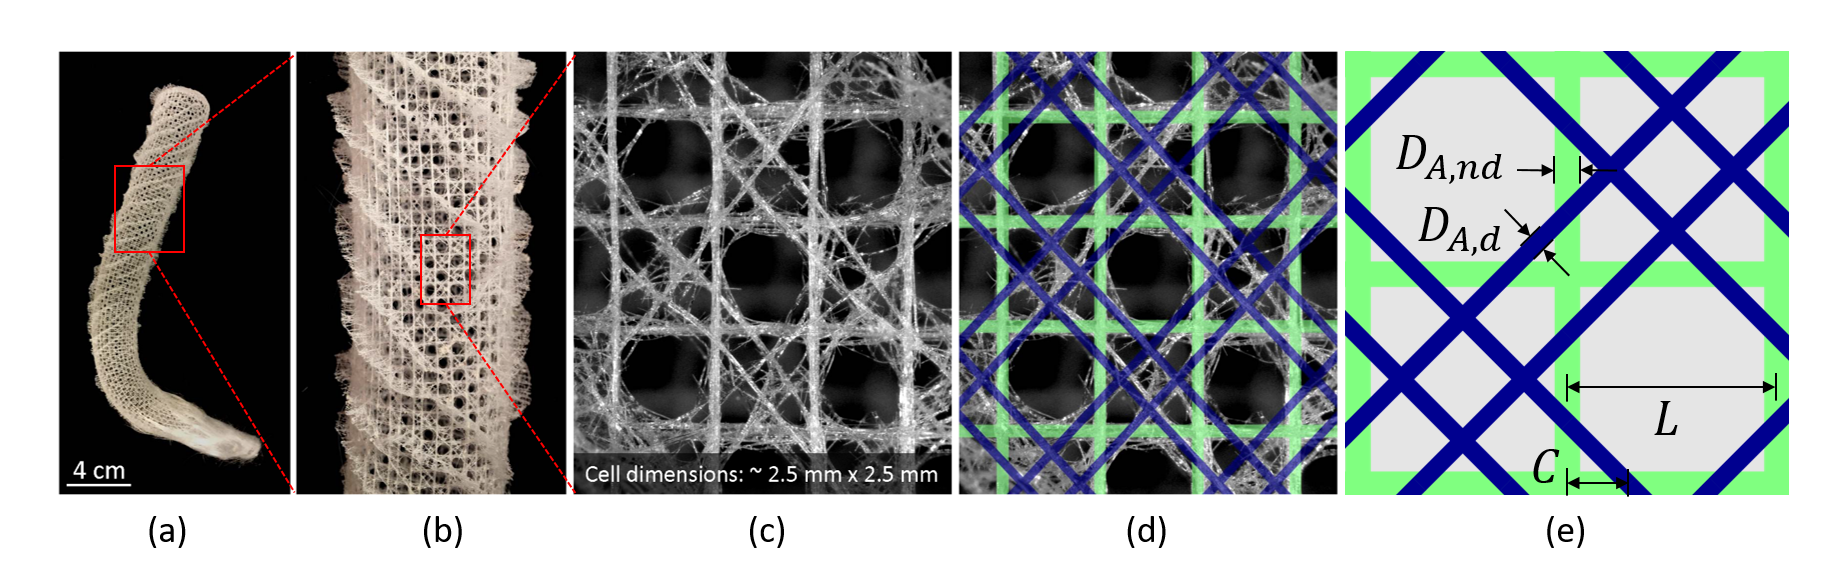
\includegraphics[width=0.9\textwidth]{Fig1}
\end{center}
\caption{\textbf{Hexactinellid sponge \textit{Euplectella aspergillum.}} (a)-(b) Full-frame photo of sponge. (c) Close up microscope image of the sponge. (d) Comparison between the idealized model (green and blue lines) and the sponge structure. (e) Representative volume element unit cell of the idealized model.}\label{Fig1}
\end{figure*}

\begin{figure*}[ht]
	\centering
	\captionsetup{width=0.8\textwidth}
	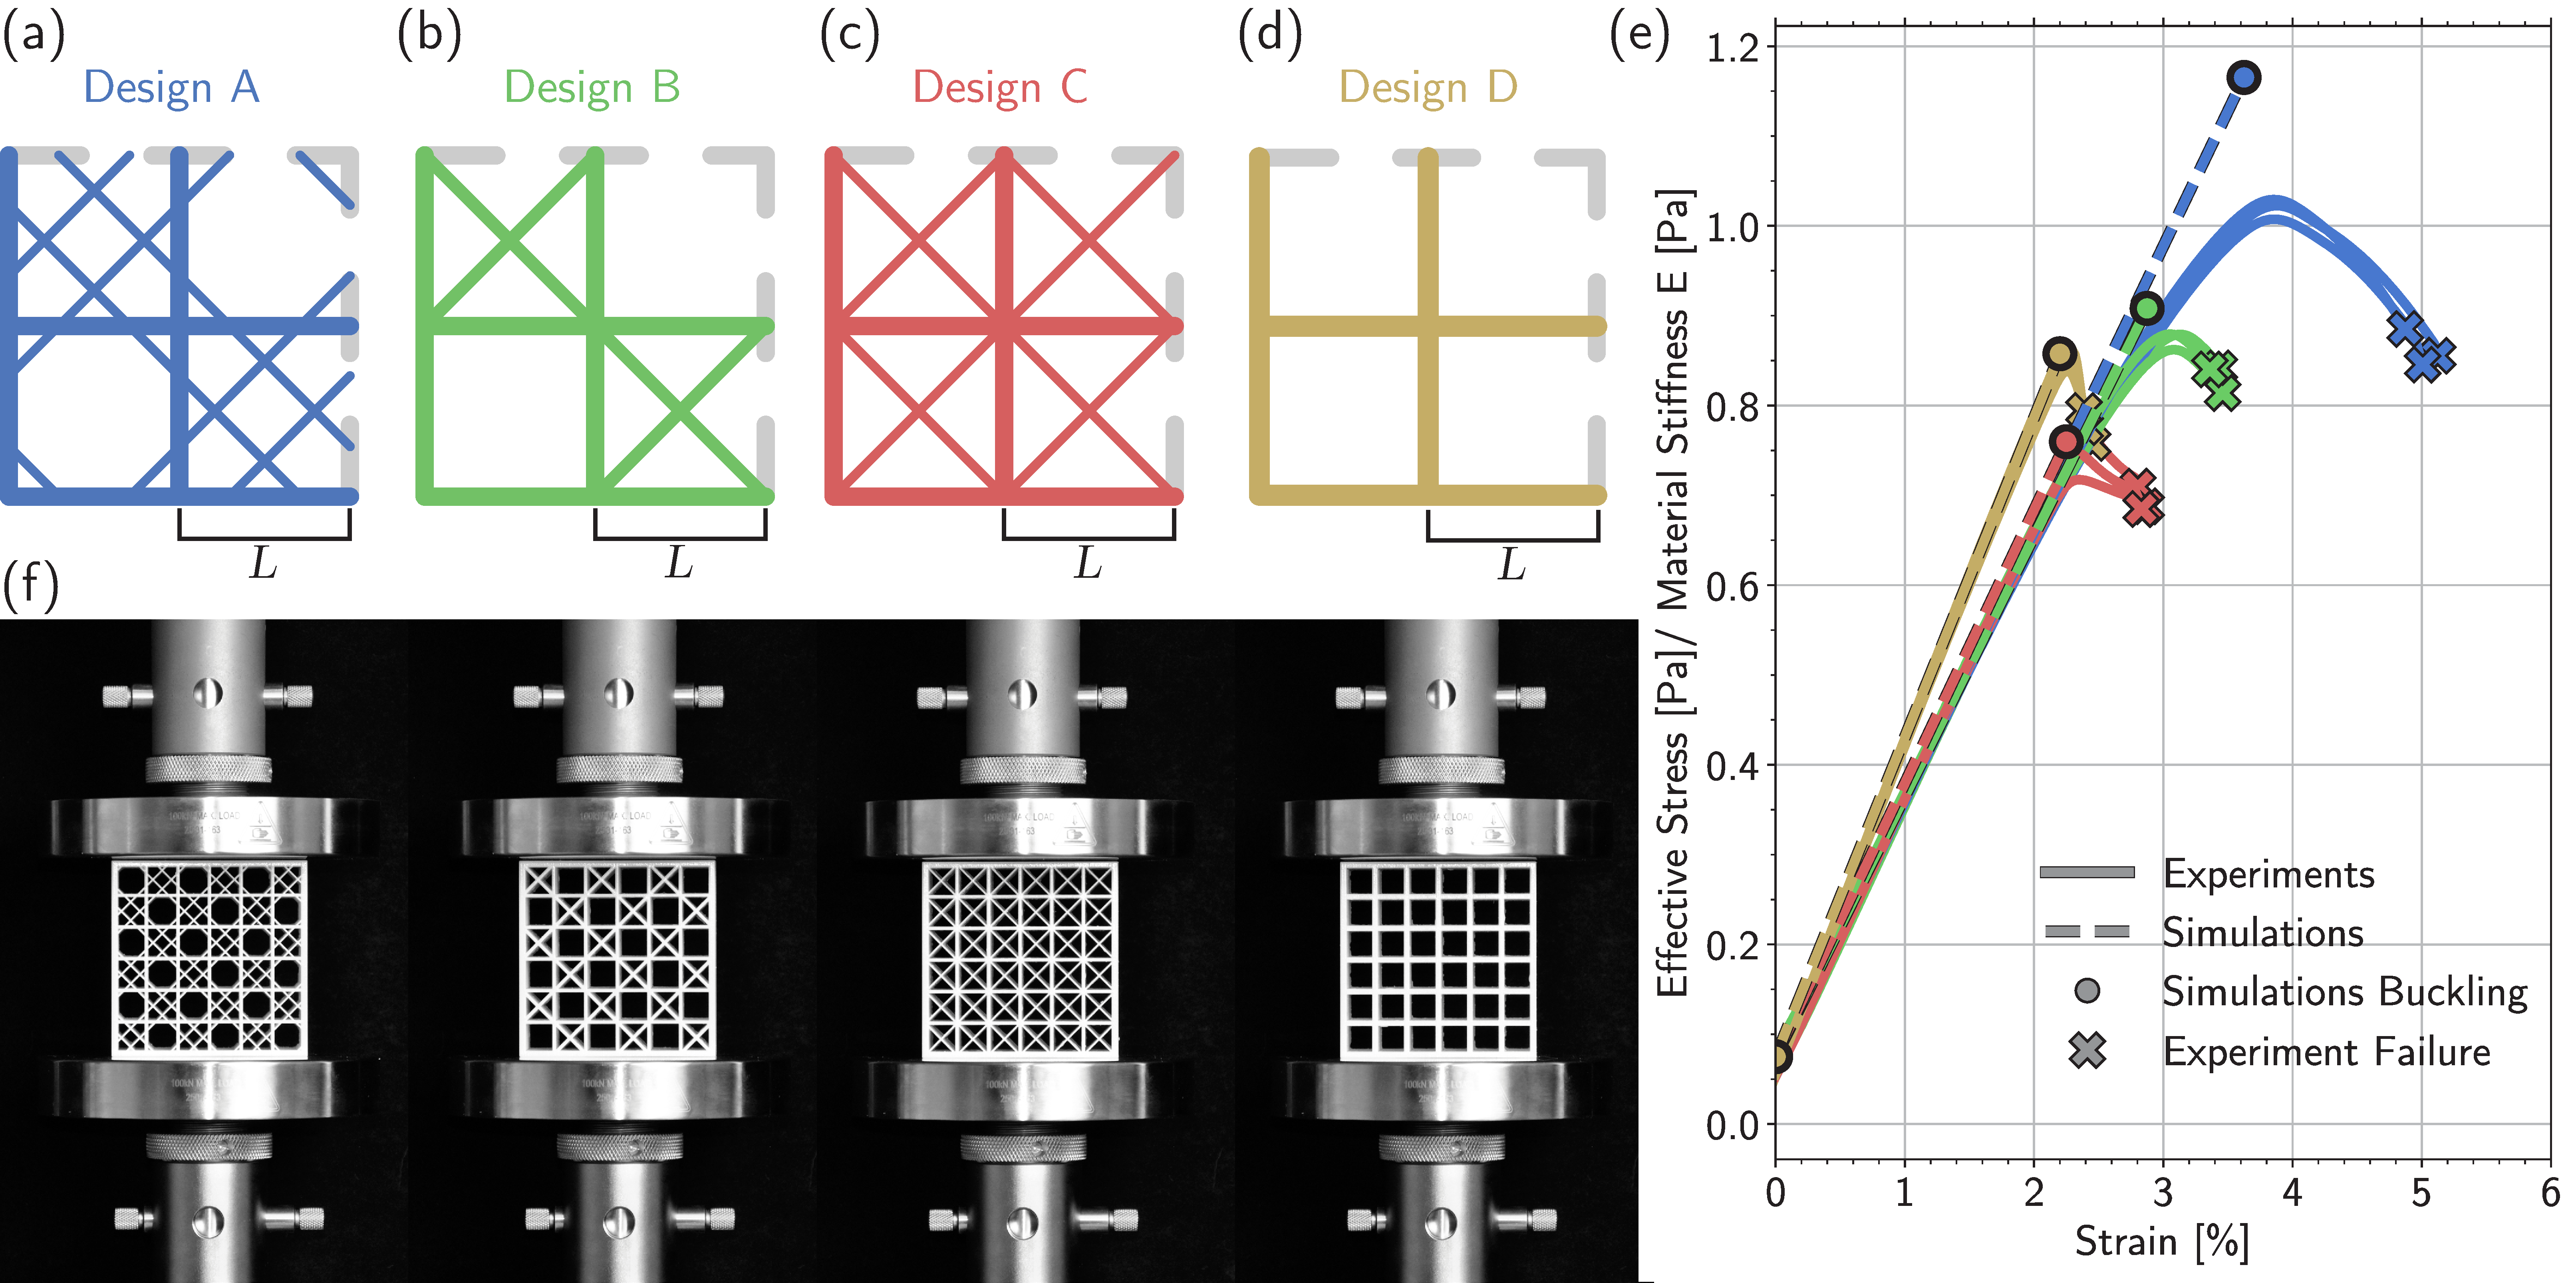
\includegraphics[width=0.9\textwidth]{Fig2}
	\caption{\textbf{Experimental Results.} (a) shows the different designs (Design A-D) considered in this analysis. (b) shows the undeformed experimental setup for the different designs. (c) shoes the post-buckling deformed state for each of the designs. (d) shows the experimental stress-strain curve as well as the overlaid numerical results for linear stiffness and critical buckling for the different designs considered.}\label{Fig2}
\end{figure*}

\begin{figure*}[ht]
	\captionsetup{width=0.8\textwidth}
	\begin{center}
		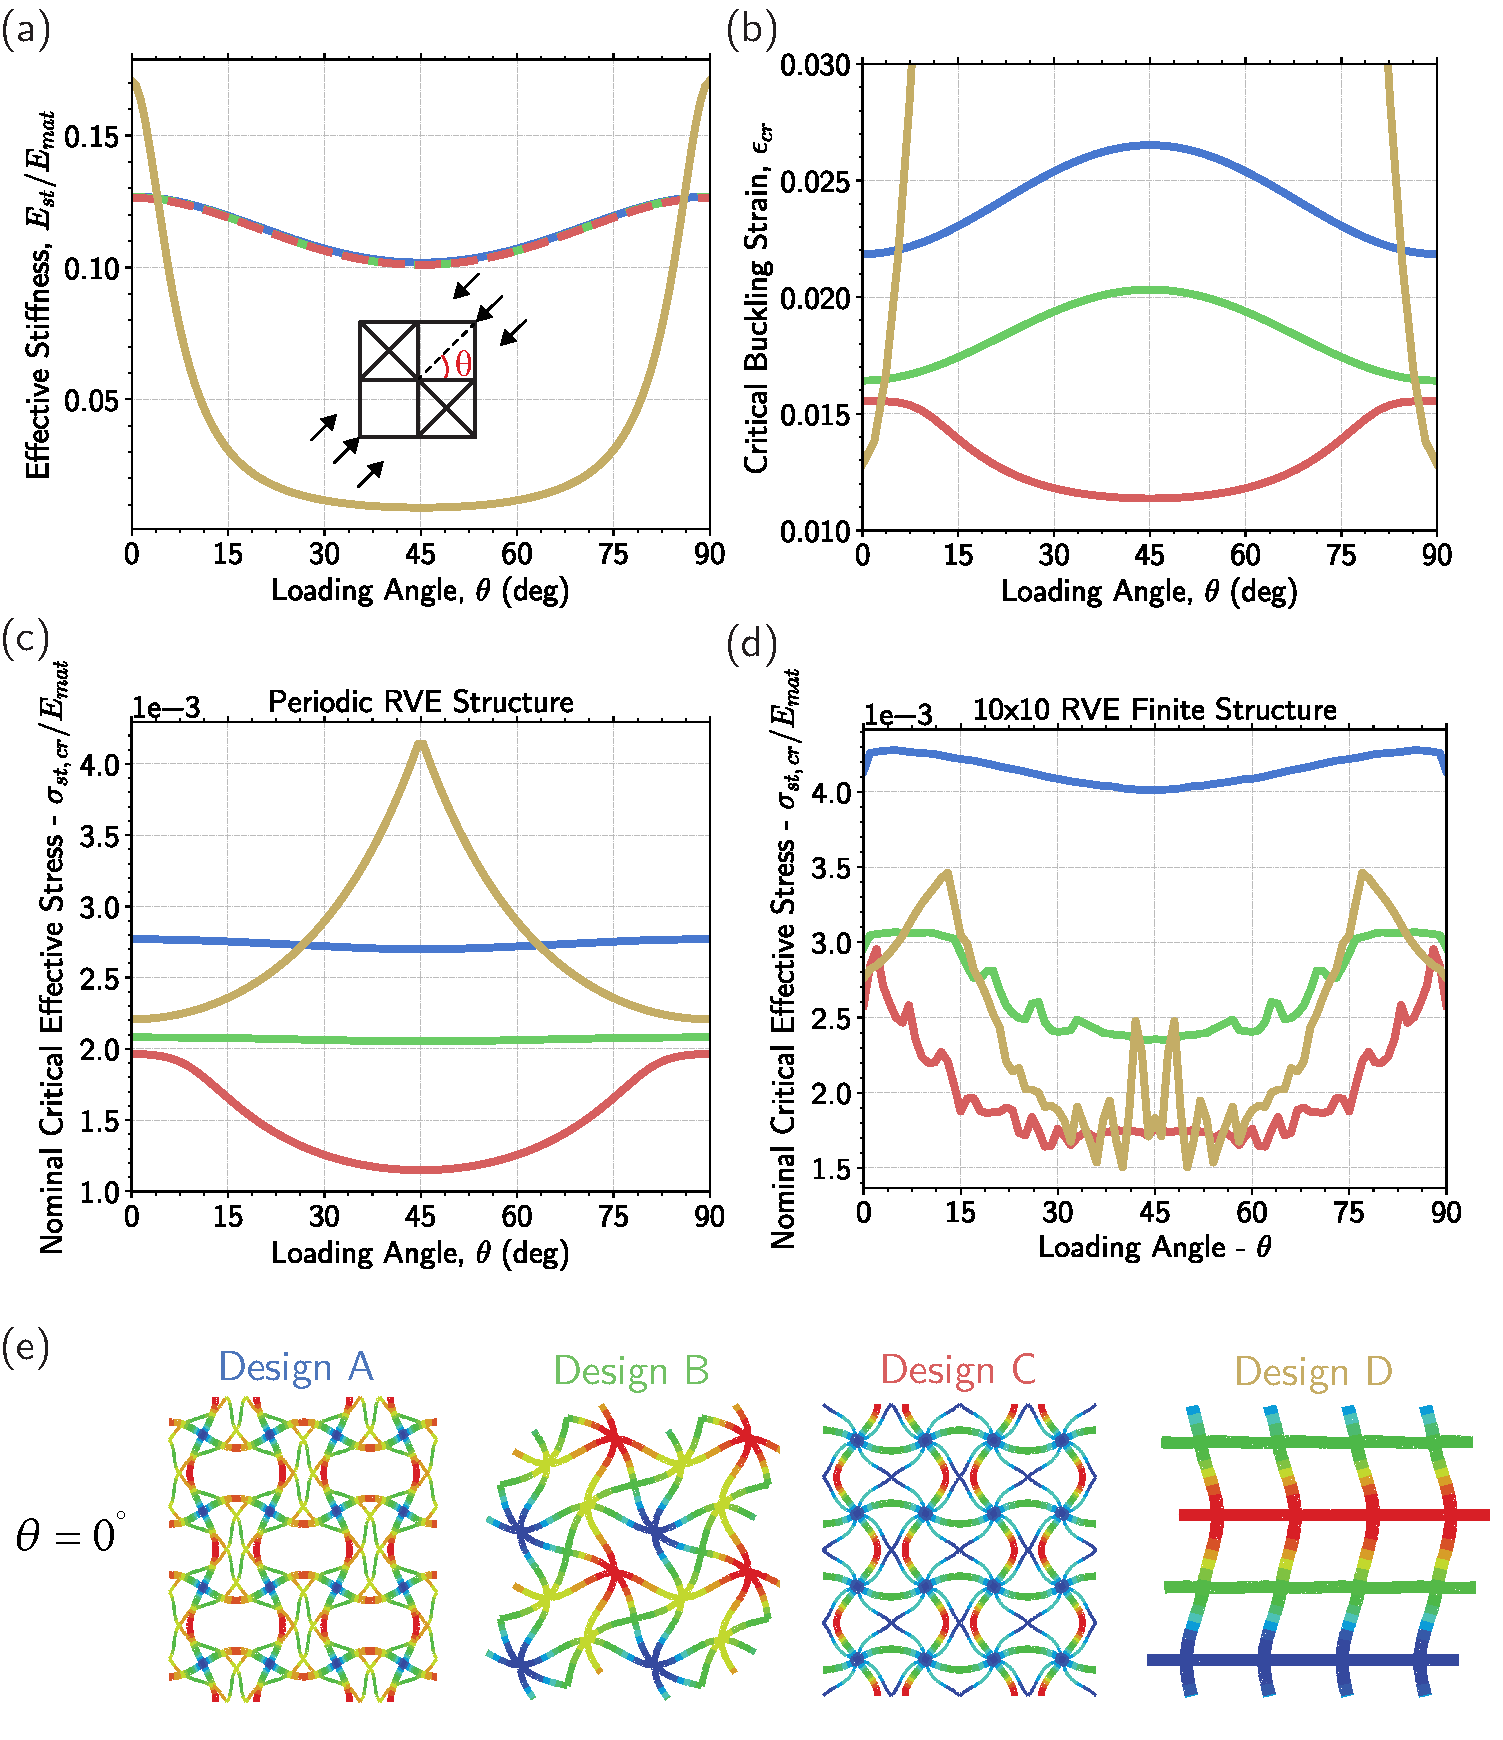
\includegraphics[width=0.7\textwidth]{Fig3}
	\end{center}
	\caption{\textbf{Structure Mechanical Response} Figure showing (a) the structural stiffness for the different designs and (b) the buckling resistance for the different designs. The designs considered are depicted below as Design A-D.} \label{Fig3}
\end{figure*}

\begin{figure*}[ht]
	\captionsetup{width=0.8\textwidth}
	\begin{center}
		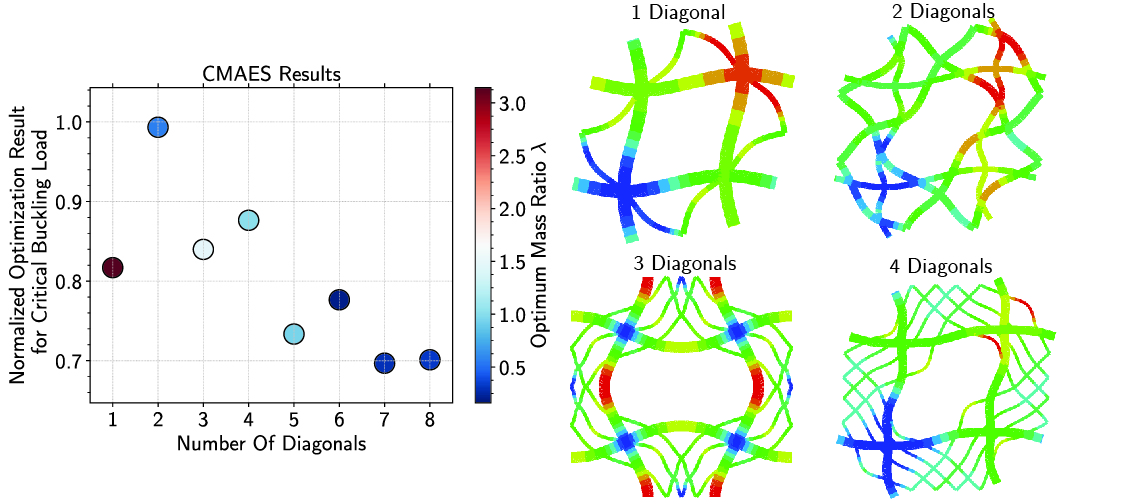
\includegraphics[width=0.7\textwidth]{Fig4}
	\end{center}
	\caption{\textbf{Critical Buckling Load Optimization Results.} (a) shows the optimal value of critical buckling load for varying number of diagonals. The color of each point represents the optimal mass ratio $\lambda$  parameter for that configuration.  Note, we do not explicitly show the other optimal values for the diagonal spacing parameters. (b) shows the resulting deformed geometries for designs including one to four diagonals.} \label{Fig4}
\end{figure*}

The design of diagonal reinforcement for truss systems found in bridges, buildings, and beam structures has not changed much since the introduction of the Long truss design patented by Colonel Long in 1830 \citep{waddell1916}. In modern day structures, we see many different iterations of new truss designs with various applications in mind but with what is the same fundamentally simple diagonal reinforcement technique. This technique, involving two diagonal trusses (one in each direction) crossing the opening of a square beam cell, limits the transverse motion of the main support beams ultimately giving the structure shear capacity and strength. Alternative, methods to strengthen beam structures have been introduced via material \hl{[...],} \mf{needs more information and citations}. However, in this study we seek to further strengthen square lattices through inspiration from a particular sponge species called \textit{Euplectella Aspergillum}, commonly known as the Venus' flower basket. This particular species, which is part of the \textit{Hexactinellid} class, is primarily made of silica and exhibit a periodic and regular grid structure with an intrinsic and different diagonal reinforcement scheme. 

\textit{Hexactinellids}, also known as glass sponges, are predominately deep sea sponges that live in ocean depths of 100-2000m. Beyond their fracture propagation inhibiting material composition \citep{weaver2007}, they are perceived to exhibit large structural rigidity and strength against buckling. 

Structurally, they are composed of a base square-grid architecture and regular ordering of vertical and horizontal struts that form the skeletal system. Furthermore, their base structure is overlaid with double diagonal (two diagonals in each direction) reinforcement struts, which create a checkerboard-like pattern of open-closed cell structure. This diagonal reinforcement design is conjectured to give the sponge greater buckling resistance and strength to localized damage then it would experience having a single diagonal reinforcement strut (with equivalent allocation of mass between the diagonal reinforcements.) 

The similarity in the structures of the sponge architecture and what we see in the Long truss design has inspired us to further explore the following research question: \textbf{Can we generate design principles for diagonal reinforcements of square beam lattices that are optimally designed to avoid global and/or local structural buckling?} 

In this paper, we present a numerical and experimental mechanical analysis of multiple  structures under various loading conditions as well as survey different arrangements within similar design space via parametric studies. Furthermore, we incorporate an optimization algorithm on our parameter space to obtain an optimal design to withstand (via critical buckling load) uniaxial loading parallel to the non-diagonal truss members. For this analysis, we restrict ourselves to four designs considered (Design A-D) that are shown along the top of \cref{Fig2}. As part of our analysis, we study the critical buckling strain and the elastic load carrying capacity of these structures. 

Numerically, we compare the linear stiffness and critical buckling strain for each of the different designs using Finite Element Analysis (FEA). To reduce the computational cost, we took advantage of the periodicity of the structures and investigated their response  by considering a Representative Volume Element (RVE) with periodic boundary conditions along the free edges of the unit cell (more information on this can be found in the SI). For our numerical model we assume Timoshenko beam elements with uniform circular cross-sections and pin-joints at beam intersections. In an effort to create a method for impartial comparison, we maintain a constant total mass (or constant volume as the material is assumed to be incompressible) between all of the designs, as well as a constant mass ratio between diagonal and non-diagonal elements for designs containing these diagonal reinforcement. 

The results presented in \cref{Fig3}(a) show that all of the structures containing diagonal reinforcement behave the same way for varying loading angles. This illustrates the fact that the structural stiffness is independent of design, but instead depend on the amount of material allocated to the perpendicular aligned beam elements. This is further supported by the graph for Design D, where all of the material from the diagonal beams is removed and allocated to the non-diagonal elements, giving the structure a higher stiffness at $0^\circ$ and lower stiffness at $45^\circ$. Any stiffness at $45^\circ$ in Design D is strictly a result of the bending resistance due to the pinned joints between the non-diagonal beams.

The results shown in \cref{Fig3}(b) indicate that the structural buckling strength is clearly dependent on the design and alignment of the beam elements. From this figure, we can see that Design A, the sponge design, has the highest buckling strength compared to the other designs containing diagonal reinforcement. At $45^\circ$ loading, Design A improves the buckling strength by a factor of 2.5 times that of Design C, which is the commonly used truss systems. 

For the experimental validation, we conducted various uniaxial compression tests of 3D printed planar beam structures (with circular cross-section) on an Instron 5566. The specimen was 3D printed using \hl{xxxx} material with manufacturer reported \hl{xxxx GPa} modulus. The printed specimen consisted of a 10x10 cell structure spanning a total of 10x10 inch planar structure. The experimental set-up consisted of two \hl{1 inch} thickness acrylic sheets bolted together along the perimeter and spaced from each other by the thickness of the 3D printed specimen.\\\\\hl{[...]} \mf{more to go here when we have experimental setup and data}

In order to study the impact of diagonal separation for Design A (sponge design), we perform a parametric study on the buckling behavior of the structure under varying separation distances ($C$). Note, we do not perform a stiffness test as the linear stiffness is not dependent on design but instead depends on the mass ratio between diagonal and non-diagonal elements as well as the diagonal element's angles. {Fig5}(a) shows the buckling behavior as a function of the non-dimensional separation ($C/L$). Where at $C/L=0$ we obtain Design B, and at $C/L=0.5$ we obtain diamond shaped reinforcement alignment. 

To investigate the effect of mass ratio on the properties of the structure, we parametrize the allocation of mass between the diagonal elements and the non-diagonal elements. To quantitatively describe this mass ratio, we introduce the variable $\lambda$ as the fraction $V_{nd}/V_d$, where $V_{nd}$ describes the collective volume of all non-diagonal elements and $V_d$ is the collective volume of all diagonal elements in the unit cell. It is important to note, that for all simulations varying $\lambda$ we maintain the same total mass of the structure, namely $V_{nd}+V_d=\mbox{const. } \forall (V_{nd},V_d)$. 



%\section*{Acknowledgments}

% No. NSF-GRFP DGE-1144152 (for M. C. F.), GEM Consortium Fellowship
% Wyss Institute for equipment. James R. Rice. Mark Scott. Joanna Aizenberg. Joost Vlassak. Chris Rycroft


\nocite{*}
\bibliography{refs}
\bibliographystyle{apalike}

\end{document}